\documentclass[11pt, a4paper]{article}

% --- Packages ---
\usepackage[T1]{fontenc}
\usepackage{lato}
\usepackage[utf8]{inputenc}
\usepackage[a4paper, margin=1in, headheight=1.5cm, headsep=0.5cm, footskip=1.5cm]{geometry}
\usepackage{fancyhdr}
\usepackage{graphicx}
\usepackage[dvipsnames, svgnames]{xcolor}
\usepackage{tcolorbox}
\usepackage{colortbl}
\tcbuselibrary{skins, breakable}
\usepackage{titlesec}
\usepackage{enumitem}
\usepackage{tabularx}
\usepackage{ragged2e}
\usepackage{amssymb}
\usepackage{hyperref}

% --- Colors (Using Green Theme) ---
\definecolor{SmaileBlue}{HTML}{00AEEF}
\definecolor{SmaileGreen}{HTML}{92D050}
\definecolor{SmaileOrange}{HTML}{ED7D31}
\definecolor{SmaileGray}{HTML}{595959}
\definecolor{SmaileLightBlue}{HTML}{E7F7FE}
\definecolor{SmaileLightGreen}{HTML}{F4FBEE}

% --- Settings ---
\tcbset{colback=white, colframe=SmaileGray, fonttitle=\bfseries}
\hypersetup{colorlinks=true, linkcolor=SmaileGreen, urlcolor=SmaileGreen}
\newcolumntype{L}{>{\RaggedRight\arraybackslash}X}

% --- Header/Footer ---
\pagestyle{fancy}
\fancyhf{}
\fancyhead[L]{
\includegraphics[height=1.2cm]{smaile_brand_assets/Logo_Co-founded_by_EU.jpeg}}
\fancyhead[R]{
\includegraphics[height=1.2cm]{smaile_brand_assets/logo_smaile_transparentbg_no_smaile.png}}
\fancyfoot[R]{\footnotesize Page \thepage}

% --- Title Formats ---
\titleformat{\section}{\normalfont\Large\bfseries\color{SmaileGreen}}{\thesection.}{1em}{}
\titleformat{\subsection}{\normalfont\large\bfseries\color{SmaileGray}}{Activity \thesubsection:}{1em}{}
\titleformat{\subsubsection}{\normalfont\normalsize\bfseries\color{SmaileGray}}{}{0em}{}

% --- Boxes ---
\newtcolorbox{keyinfobox}{colback=SmaileLightGreen, colframe=SmaileGreen, title=Key Information, fonttitle=\bfseries\color{SmaileGreen}, enhanced, attach boxed title to top left={yshift=-2mm, xshift=3mm}}
\newtcolorbox{eurobox}{colback=SmaileLightBlue, colframe=SmaileBlue, title=European Dimension / Erasmus+ Connection, fonttitle=\bfseries\color{SmaileBlue}, enhanced, attach boxed title to top left={yshift=-2mm, xshift=3mm}, breakable}

\begin{document}

\title{\textbf{\color{SmaileGreen}A Bite of Future}}
\author{SMaiLE Project}
\date{}
\maketitle
\thispagestyle{plain}

% --- Key Info ---
\begin{keyinfobox}
    \begin{description}[leftmargin=*, labelindent=0pt]
        \item[\bfseries\color{SmaileGreen} Target Group:] 4 - 7 y.o.
        \item[\bfseries\color{SmaileGreen} Duration:] 40 min
    \end{description}
    \textbf{Key Learning Goals:}
    \begin{enumerate}
        \item \textbf{Food Importance:} Understand why we need food to grow and be healthy.
        \item \textbf{Origin:} Discover that food comes from farms, gardens, and even labs.
        \item \textbf{Future Thinking:} Think about new ways of growing food to feed everyone.
        \item \textbf{Creativity:} Use imagination to design fun and healthy future meals.
        \item \textbf{Collaboration:} Work in teams to share ideas.
    \end{enumerate}
\end{keyinfobox}

% --- Outcomes ---
\section*{Learning Outcomes}
Students will be able to:

\subsubsection*{KNOWLEDGE \& UNDERSTANDING:}
\begin{itemize}
    \item Understand that AI and robots help grow, pick, and package food.
    \item Recognize simple tasks machines can do with AI guidance.
    \item Understand the concept of ``smart machines'' or ``robot helpers''.
\end{itemize}

\subsubsection*{SKILLS \& ABILITIES:}
\begin{itemize}
    \item Role-playing and dramatic play skills.
    \item Simple decision-making (e.g., ``If plant is droopy $\to$ water it'').
    \item Drawing and storytelling to express creative ideas.
\end{itemize}

\subsubsection*{ATTITUDES \& VALUES:}
\begin{itemize}
    \item Show curiosity about how food is made.
    \item Appreciate teamwork and shared responsibility.
    \item Value technology as a helpful tool when used wisely.
\end{itemize}

% --- EU Connection ---
\begin{eurobox}
\begin{itemize}
    \item \textbf{Early STEM:} Promotes digital education in line with European priorities.
    \item \textbf{Sustainability:} Encourages awareness of food security and innovation.
    \item \textbf{Key Competences:} Supports cultural awareness and digital literacy.
    \item \textbf{Global Challenges:} Introduces technology's role in sustainable food production.
\end{itemize}
\end{eurobox}

\newpage
% --- Resources ---
\section{Resources and Tools}
\begin{itemize}
    \item \textbf{Story:} ``Farmer Ella and the Robot Helpers''.
    \item \textbf{Props:} Fruit/vegetable images, watering can, baskets.
    \item \textbf{Materials:} Robot and AI name tags, Drawing paper, crayons/markers.
    \item \textbf{Cards:} Weather and crop condition cards (sun, rain, ripe fruit).
\end{itemize}

\subsubsection*{Classroom Support Materials}
\begin{itemize}
    \item Use teacher-led slides or printed picture prompts to introduce Farmer Ella and the robot helpers.
\end{itemize}

% --- Activity Overview ---
\section*{Activity Overview}
\begingroup
\small
\begin{tabularx}{\textwidth}{|l|l|L|}
    \hline
    \rowcolor{SmaileLightGreen} \textbf{Phase} & \textbf{Time} & \textbf{Activity} \\ \hline
    Intro & 10 min & \textbf{Storytime:} Read ``Farmer Ella'' story. Explain AI simply as a ``smart computer brain''. \\ \hline
    Research & 20 min & \textbf{Role-Play:} ``Farmer Ella's Smart Farm''. Students act as Robots, Plants, and AI. \\ \hline
    Creative & 15 min & \textbf{Design:} ``Design Your Own Food Robot''. Drawing activity. \\ \hline
    Reflection & 10 min & \textbf{Circle Time:} Sharing what was learned. Emoji voting. Coloring activity. \\ \hline
\end{tabularx}
\endgroup

% --- Activities ---
\section{Introduction and Motivation}
\textbf{Goal:} Introduce the story and concept.
\begin{itemize}
    \item Teacher reads the story \textit{Farmer Ella and the Helpful Robots}.
    \item \textbf{Story Summary:} Farmer Ella uses robots like Picksy (picker) and Sprinkles (waterer), guided by Brainy (AI), to run a smart farm efficiently.
    \item \textbf{Discussion:} ``Who helps grow your food?'' ``What do you think robots can do on a farm?''
\end{itemize}

\begin{center}
    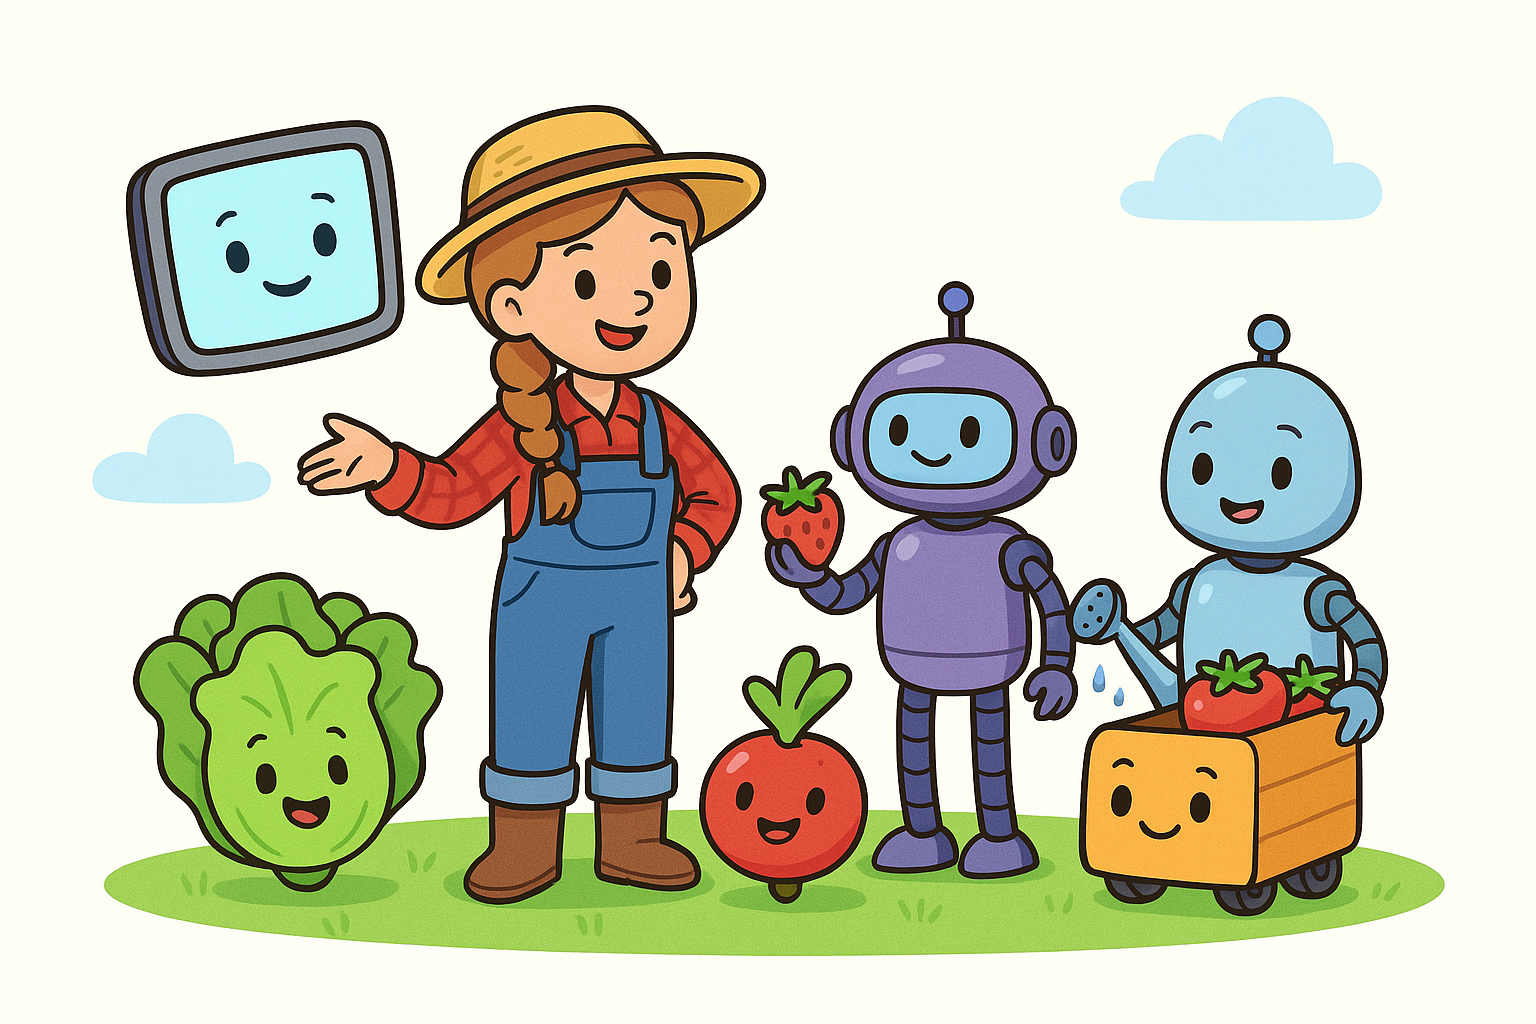
\includegraphics[width=0.7\textwidth]{images/scenario_bite_future_4-7_img1.png}
\end{center}

\section{Research and Learning}
\subsection{Role-Play: Farmer Ella's Smart Farm}
\textbf{Setup:} Transform classroom into a farm.
\begin{itemize}
    \item \textbf{Roles:} Plants (lettuce/strawberries), Robots (Picksy/Sprinkles), AI (Brainy).
    \item \textbf{Action:} The AI student gives commands based on clues.
    \item \textbf{Examples:}
    \begin{itemize}
        \item ``Only water the plants that are droopy.''
        \item ``Pick the strawberries that are red.''
        \item ``Don't water today, it's raining!''
    \end{itemize}
    \item \textbf{Goal:} Build logic and connection to real AI thinking (Cause \& Effect).
\end{itemize}

\section{Creative Application}
\subsection{Design Your Own Food Robot}
Each child creates their own food robot helper on paper.
\begin{itemize}
    \item \textbf{Prompts:} What is your robot's name? What job does it do?
    \item \textbf{Sentence Starter:} ``My robot helps by...''
    \item \textbf{Display:} Create a classroom wall titled ``Our Food Robots''.
\end{itemize}

\section{Reflection and Evaluation}
\subsection{Class Reflection Circle}
\begin{itemize}
    \item Ask: ``What was it like to be the AI or robot?''
    \item Emoji Voting: Did you enjoy the activity?
    \item \textbf{Coloring:} Complete the ``Brainy AI'' coloring page (see image below).
\end{itemize}

\begin{center}
    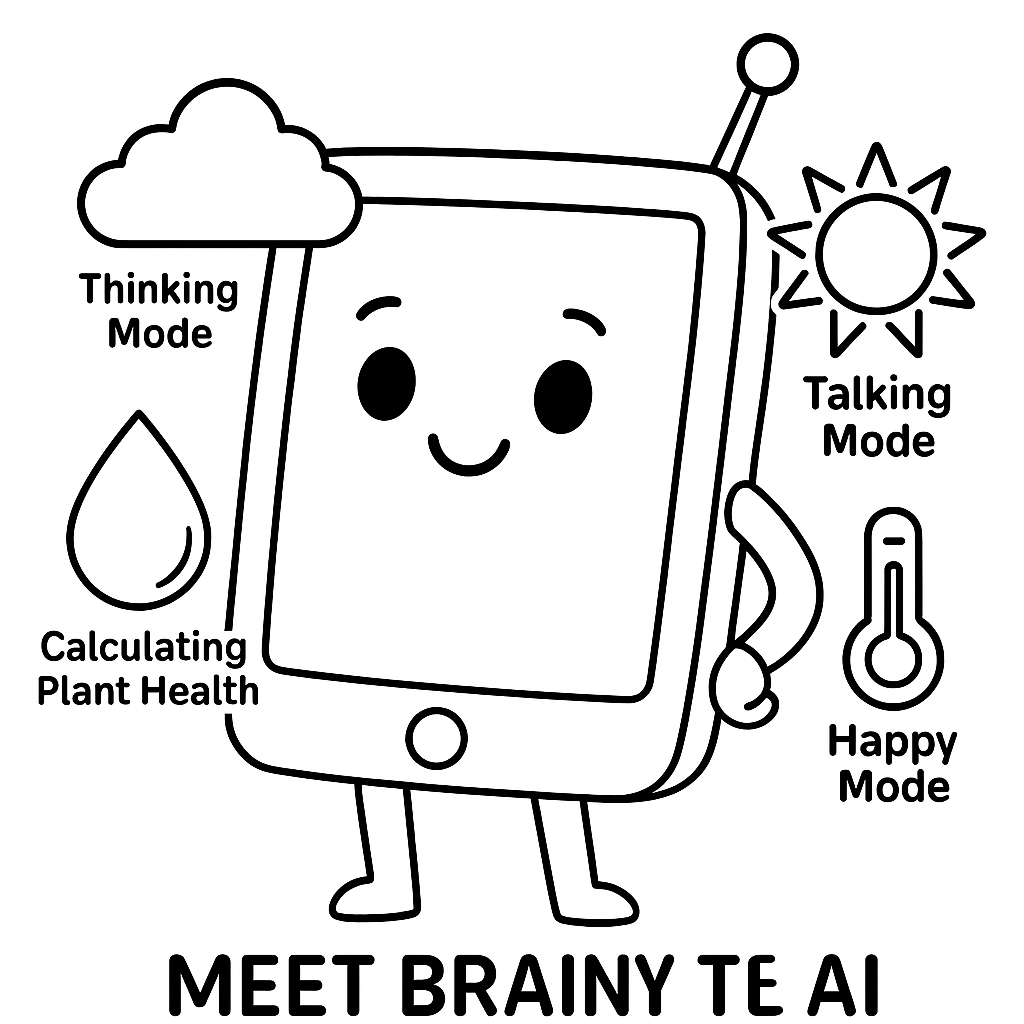
\includegraphics[width=0.5\textwidth]{images/scenario_bite_future_4-7_img2.png}
\end{center}

\end{document}
